\documentclass[border=10pt]{standalone}

\usepackage{tikz}
\usepackage{tikzsymbols}
\usetikzlibrary{calc,patterns,shapes.geometric}

\def\centerarc[#1](#2)(#3:#4:#5){\draw[#1] ($(#2)+({#5*cos(#3)},{#5*sin(#3)})$) arc (#3:#4:#5);}

\begin{document}
	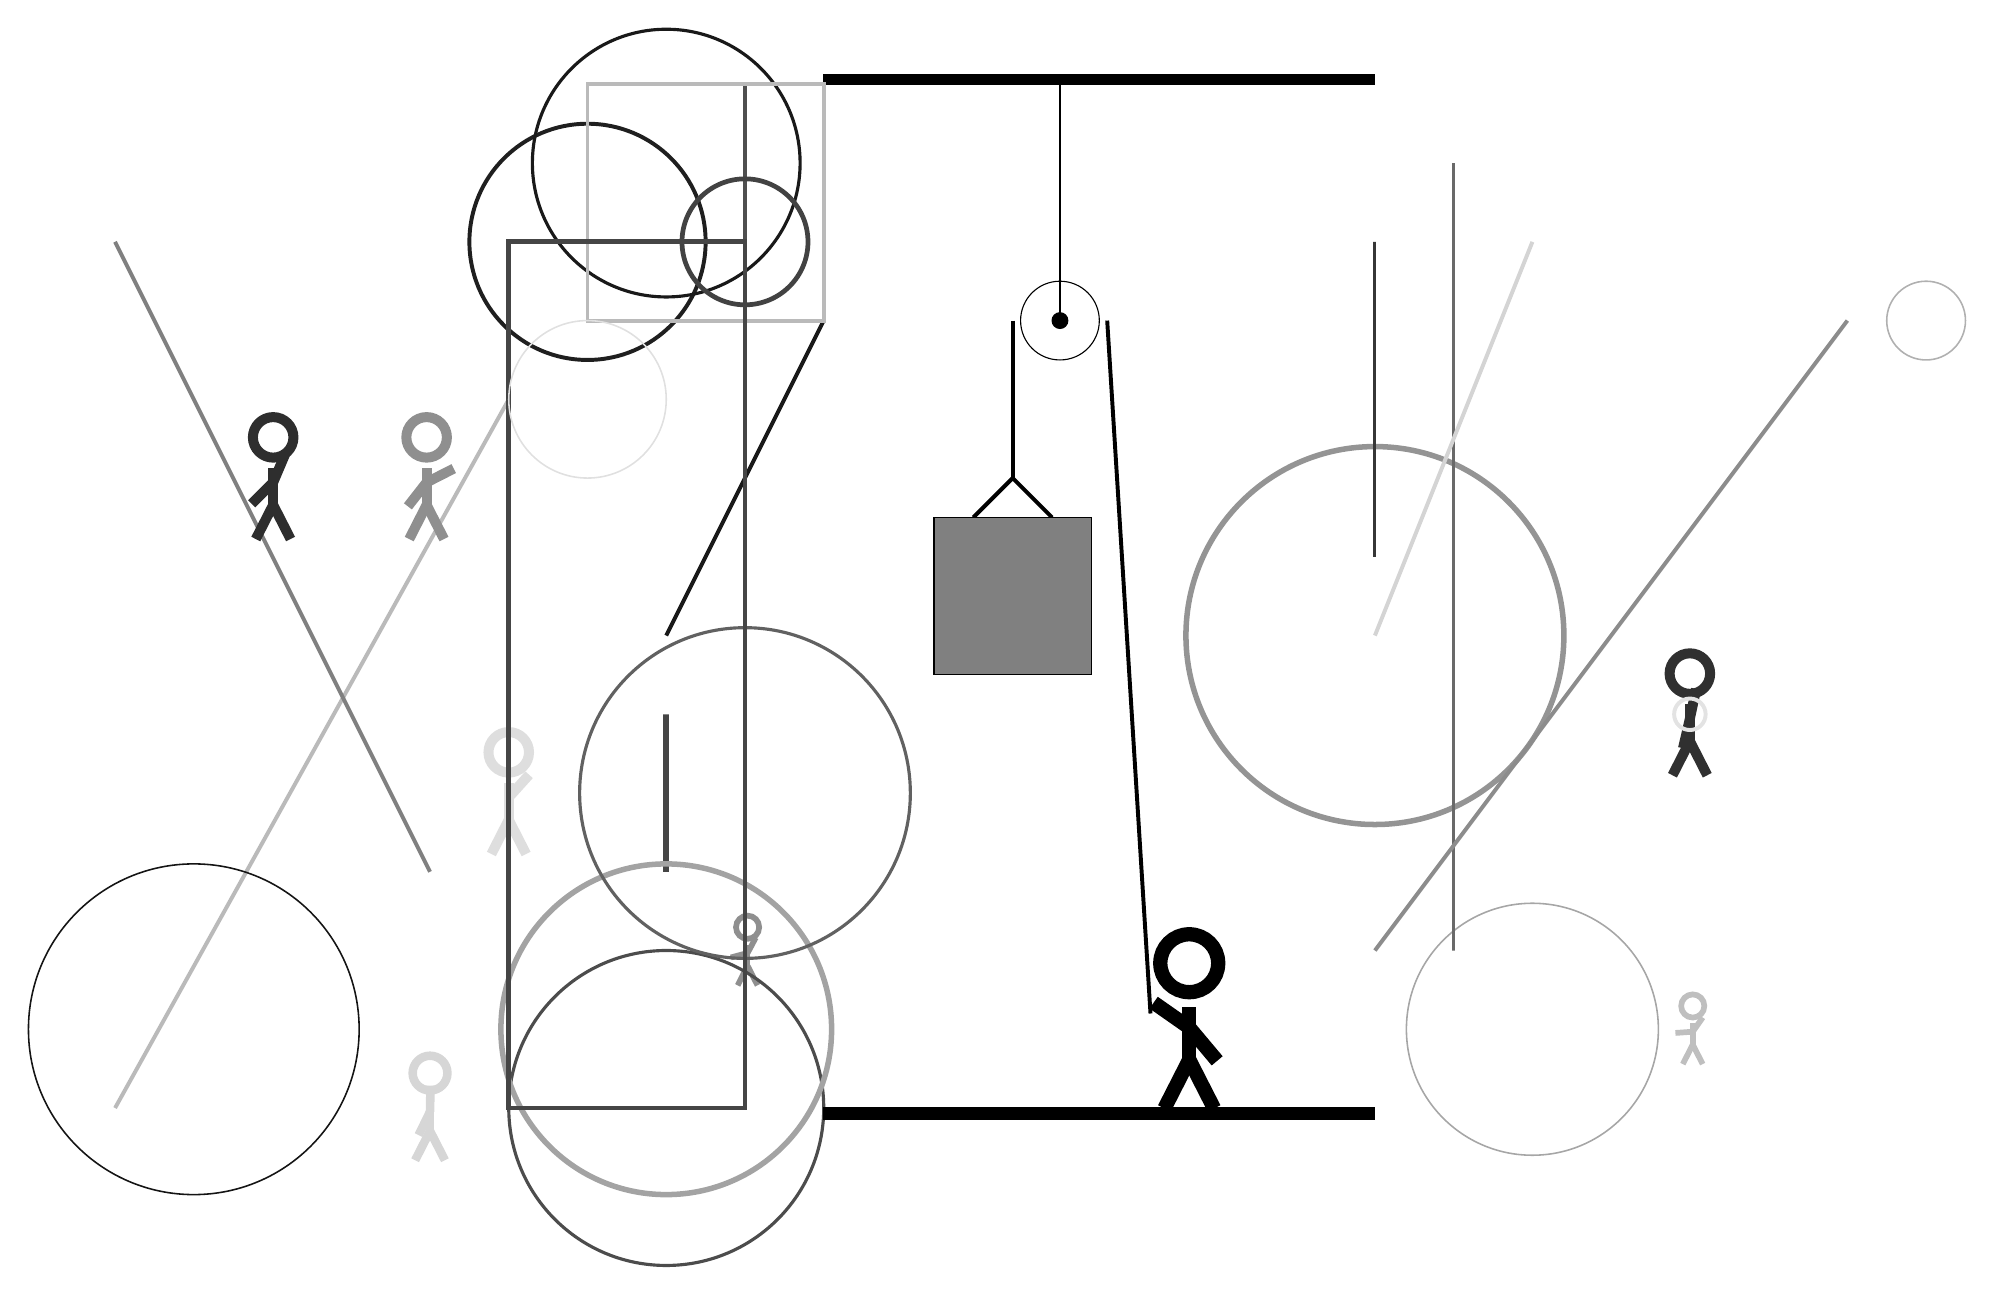
\begin{tikzpicture}
		%%%%% START %%%%%
		
		\draw[fill=black] (-2, 10) rectangle (5, 10.125);
		
		\draw[line width=0.7mm, color=black!73] (-4, 2) rectangle (-4, 0);
		
		\node[line width=0.5mm, color=black!13] at (-6, 1) {\Strichmaxerl[7][90][48]};
		\draw[line width=0.5mm, color=black!27](-6, 6) -- (-11, -3);
		\draw[line width=0.5mm, color=black!90](-4, 3) -- (-2, 7);
		\draw[line width=0.5mm, color=black!69](-3, 10) -- (-3, -3);
		\draw[line width=0.5mm, color=black!50](-7, 0) -- (-11, 8);
		\node[line width=0.5mm, color=black!44] at (-3, -1) {\Strichmaxerl[4][15][62]};
		
		\draw [line width=0.2mm, color=black!35](7, -2) circle (1.6);
		\node[line width=0.6mm, color=black!81] at (9, 2) {\Strichmaxerl[7][77][78]};
		\draw [line width=0.5mm, color=black!88](-5, 8) circle (1.5);
		\draw [line width=0.7mm, color=black!42](5, 3) circle (2.4);
		\node[line width=0.5mm, color=black!16] at (-7, -3) {\Strichmaxerl[6][64][89]};
		\node[line width=0.6mm, color=black!25] at (9, -2) {\Strichmaxerl[4][4][55]};
		\draw [line width=0.4mm, color=black!90](-4, 9) circle (1.7);
		\draw[line width=0.3mm, color=black!59] (6, -1) rectangle (6, 9);
		\draw [line width=0.6mm, color=black!74](-3, 8) circle (0.8);
		
		\draw [line width=0.5mm, color=black!11](9, 2) circle (0.2);
		\draw[line width=0.4mm, color=black!79] (5, 4) rectangle (5, 8);
		\draw [line width=0.4mm, color=black!70](-4, -3) circle (2.0);
		
		\node[line width=0.3mm, color=black!44] at (-7, 5) {\Strichmaxerl[7][52][27]};
		\draw [line width=0.2mm, color=black!31](12, 7) circle (0.5);
		
		\draw[line width=0.5mm, color=black!45](5, -1) -- (11, 7);
		\draw[line width=0.5mm, color=black!27] (-2, 7) rectangle (-5, 10);
		\draw [line width=0.2mm, color=black!92](-10, -2) circle (2.1);
		\node[line width=0.5mm, color=black!82] at (-9, 5) {\Strichmaxerl[7][45][67]};
		\draw [line width=0.7mm, color=black!36](-4, -2) circle (2.1);
		\draw[line width=0.5mm, color=black!17](5, 3) -- (7, 8);
		\draw [line width=0.4mm, color=black!62](-3, 1) circle (2.1);
		
		\draw[line width=0.6mm, color=black!73] (-3, 8) rectangle (-6, -3);
		
		\draw [line width=0.2mm, color=black!12](-5, 6) circle (1.0);
		
		\draw (1, 7) circle (0.5);
		\draw[fill=black] (1, 7) circle (0.1);
		\draw (1, 10) -- (1, 7);
		
		\draw[line width=0.5mm] (-0.1, 4.5) -- (0.4, 5.0) -- (0.9, 4.5);
		\draw[fill=black!50] (-0.6, 4.5) rectangle (1.4, 2.5);
		
		\draw[line width=0.5mm] (0.4, 7) -- (0.4, 5.0);
		\centerarc[line width=0.5mm](1, 7)(0:180:0.6);
		\draw[line width=0.5mm](1.6, 7) -- (2.15, -1.8);
		
		\node at (2.6, -1.9) {\Strichmaxerl[10][-35][-50]};
		
		\draw[fill=black] (-2, -3) rectangle (5, -3.15);
		
		%%%%% END %%%%%
	\end{tikzpicture}
\end{document}